% % % Set the style for this file:
\pagestyle{standard}

% % % Beginning of the chapter
\chapter{Infrared thermograms analysis}\label{chapter3}

	% % % Set the style for the first page:
	\thispagestyle{chapter-first-page}

	\section{Factors affecting the IR measurements.}\label{section3.1}
	
		When we take an IR picture of any object at room temperature, for instance, we intuitively expect the entire image to be of only one color (corresponding to the ambient temperature). However, this is rarely the case. There  are several factors that can make the IR temperature readings to move away from the real values, the most important are:
		
		\begin{enumerate}[label={\arabic*)}]
			\item Different emissivity values of the objects in the image.
			\item Reflectivity and Transmissivity of the object.
			\item Spectral Response Function of the IR camera in the wavelength range in which it operates.
			\item Ambient conditions. Apparent reflected temperature.
			\item Viewing angle of the IR camera with respect to the object.
		\end{enumerate}
		
		To understand how all this factors come into play we can imagine the following situation (Figure \ref{fig3.1}).  Let's assume that we have a target which is placed in front of a generic IR sensor. We are interested in measure the amount of radiation coming from the target due to emission alone, since this will be the only measure of the “real” temperature of our object. Form Equations \ref{eq1.1} and \ref{eq1.4} we can estimate the amount of emitted IR radiation as: 
		
		\begin{equation}\label{eq3.1}
			\varepsilon(\lambda,T) \cdot N_{b}(\lambda,T)
		\end{equation}	
		
		Here $T$ is the actual (real) temperature of the target. In addition, we will have two more contributions to the amount of IR radiation flying in the direction of the sensor. This other contributions are produced by additional sources of heat. 
		The first is the amount of radiation coming from external heat sources that is reflected in the target surface. This contribution is given by:
		
		\begin{equation}\label{eq3.2}
			\rho(\lambda,T) \cdot N_{b}(\lambda,T_{r})
		\end{equation}	
	
		Where $T_{r}$ is the \textit{apparent reflected temperature} of the target surface. This is an irreducible source of IR background, even with an isolated thermal chamber, and is therefore always present in the estimation of the real surface temperature. In this sense, we can regard the interior walls of the isolation chamber (and all other equipment inside) as "external" heat sources and, as the temperature of such objects should be close to the room temperature, this apparent reflected temperature is often taken as the ambient temperature. We will discuss further on this temperature and its estimation method in the next paragraph.
		The second source of additional IR radiation is that part of the radiation coming from a heat source behind the target that is transmitted through the target itself. This contribution is determined as:
		
		\begin{equation}\label{eq3.3}
			\tau(\lambda,T) \cdot N_{b}(\lambda,T_{t})
		\end{equation}	
		
		Where $T_{t}$ is the \textit{apparent transmitted temperature}. This source of IR background can be avoided by place the target in a thermal enclosure (chamber), leaving all external heat sources outside. However, for complex objects (as the Petal) composed by layers of different materials, this factor can appear if, for example, the surface material (facing the IR sensor) is somewhat transmissive and the heat from other layers reaches them and passes through.
		
		\begin{figure}[ht!]
			\centering
			\captionsetup{justification=centering,margin=2cm}
			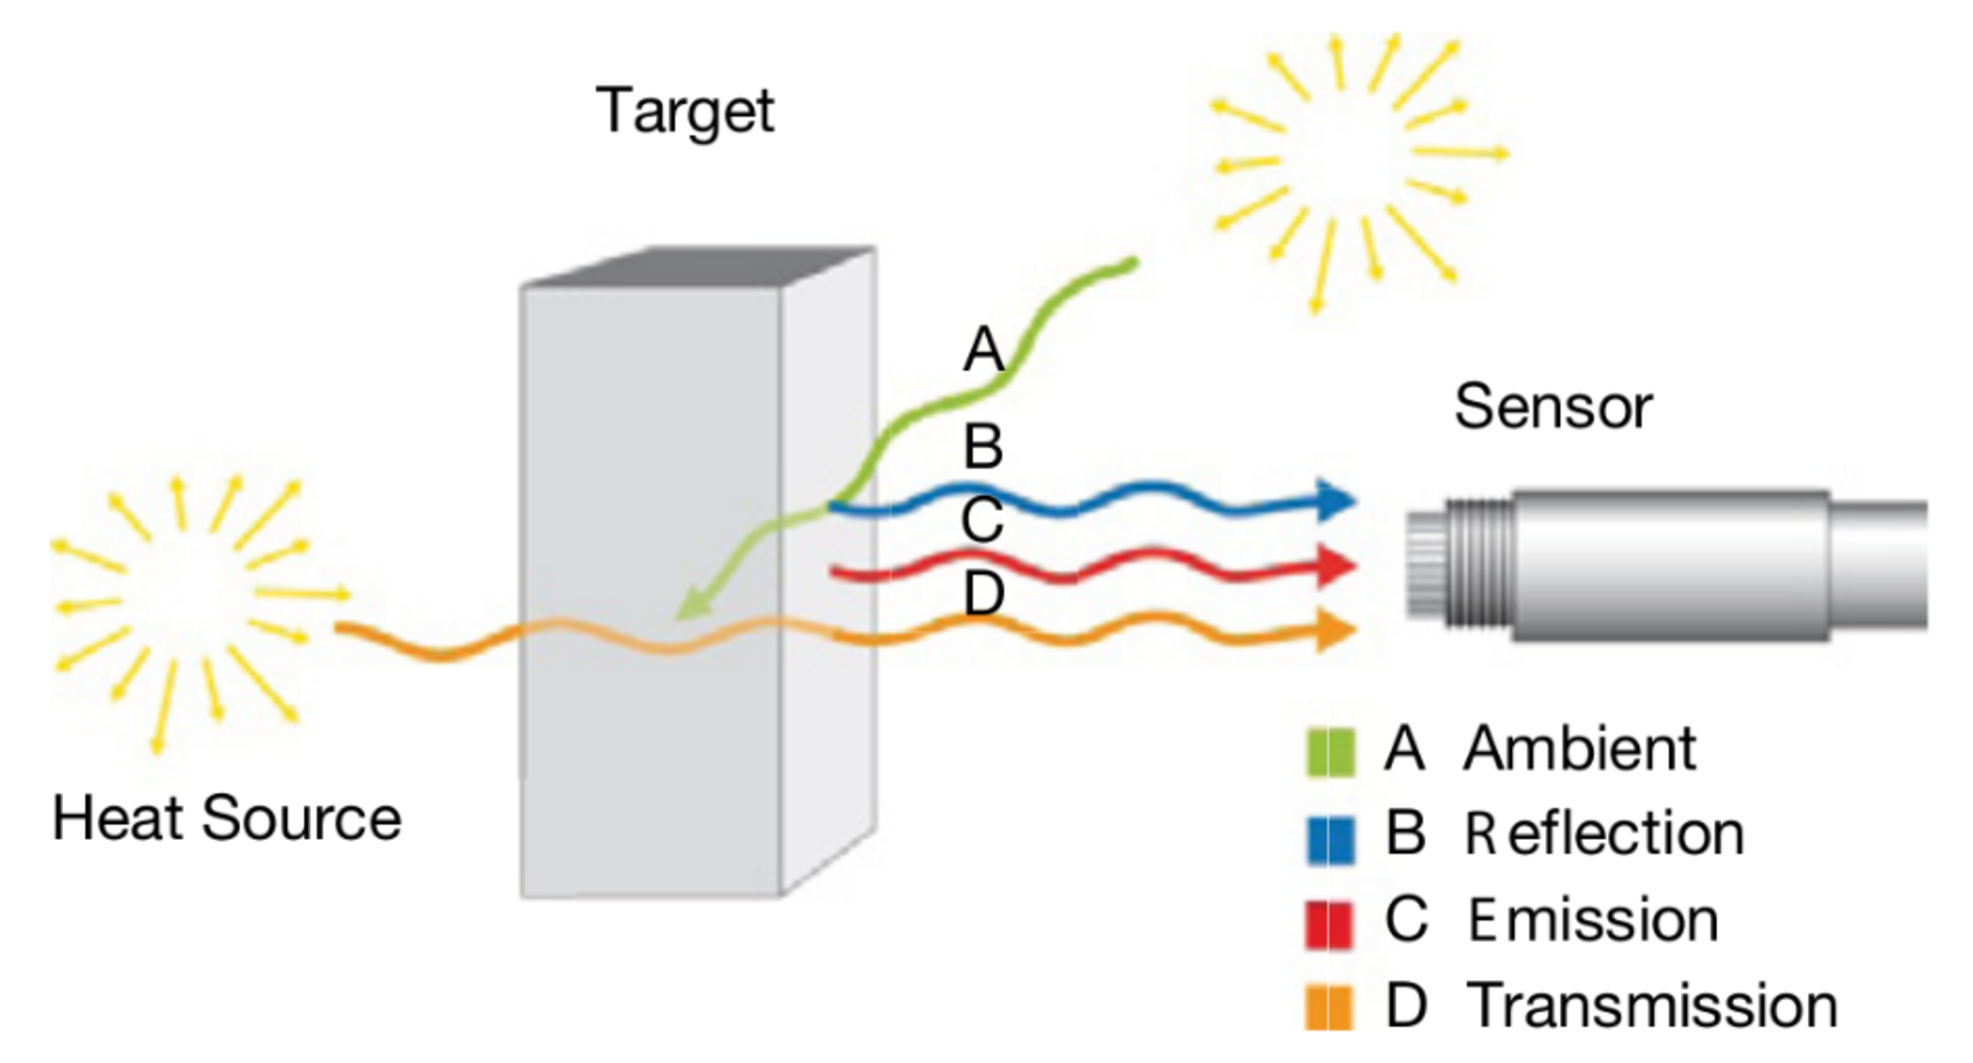
\includegraphics[scale=0.30]{Figures/Chapter03/SchematicsOfIRRadiation.pdf}
			\caption{Schematics of the IR radiation interaction with a target surface: (A) radiation from an external source being partially absorbed by the target, (B) part of the radiation from A which is reflected in the direction of the IR camera, (C) thermal  radiation emitted from the target and (D) external source radiation transmitted through the target.}\label{fig3.1}
		\end{figure}
		
		The combination of all three of this factors is then the total amount of IR radiation emanating from the target surface per unit of time and area. Neglecting the transmission component, this amount is:
		
		\begin{equation}\label{eq3.4}
			N_{total}(\lambda,T)=\varepsilon(\lambda,T) \cdot N_{b}(\lambda,T)+ [1- \varepsilon(\lambda,T)] \cdot N_{b}(\lambda,T_{r})
		\end{equation}	
		
		Where we have used Equation \ref{eq1.7} to express everything in terms of emissivity. If we also consider that this $N_{total}(\lambda,T)$ is not attenuated in the air path to the IR sensor then the emissive power registered by the sensor is:
		
		\begin{equation}\label{eq3.5}
			N_{meas}(\lambda,T)= R(\lambda) \cdot N_{total}(\lambda,T)
		\end{equation}	
		
		Where $R(\lambda)$ is the sensor's \textit{Spectral Response Function}, also known as Filter Function, accounting for the fact that the sensor is intrinsically not 100\% efficient in processing the incoming spectral power nor in the entire wavelength spectrum. As mentioned in Chapter 2, our IR camera is sensitive only in the spectral range from 7.5 $\mu$m to 14 $\mu$m, but even in that range it's also not 100\% sensitive to the incoming radiation. 
		To obtain then the total (for all wavelengths) signal processed by the IR sensor we have to integrate Equation \ref{eq3.5} over the wavelength range that our sensor is sensitive to (from $\lambda_{1}$=7.5 $\mu$m to $\lambda_{1}$=14 $\mu$m):
		
		\begin{equation}\label{eq3.6}
			N_{meas}(T)= \int_{\lambda_{1}}^{\lambda_{2}} N_{meas}(\lambda,T) d\lambda = \int_{\lambda_{1}}^{\lambda_{2}} R(\lambda) \cdot N_{total}(\lambda,T) d\lambda
		\end{equation}		
		
		\begin{equation}\label{eq3.7}
			N_{meas}(T)= \int_{\lambda_{1}}^{\lambda_{2}} R(\lambda) \cdot \varepsilon(\lambda,T) \cdot N_{b}(\lambda,T) d\lambda + \int_{\lambda_{1}}^{\lambda_{2}} R(\lambda) \cdot [1- \varepsilon(\lambda,T)] \cdot N_{b}(\lambda,T_{r}) d\lambda
		\end{equation}	
		
		As we don't know the functional form of $R(\lambda)$ or $\varepsilon(\lambda,T)$ we can come around this by applying the integral mean value theorem and use their average instead, as mentioned in Chapter 1. Since both $R(\lambda)$ and $\varepsilon(\lambda,T)$ should be slow-varying functions of the wavelength, there must be certain value $\xi\in [\lambda_{1},\lambda_{2}]$ such that we can express then Equation \ref{eq3.7} as:
		
		\begin{equation}\label{eq3.8}
			N_{meas}(T)= R(\xi) \cdot \varepsilon(\xi,T) \cdot \int_{\lambda_{1}}^{\lambda_{2}} N_{b}(\lambda,T) d\lambda + R(\xi) \cdot [1- \varepsilon(\xi,T)] \cdot \int_{\lambda_{1}}^{\lambda_{2}} N_{b}(\lambda,T_{r}) d\lambda
		\end{equation}	
		
		\begin{equation}\label{eq3.9}
			N_{meas}(T)= R \cdot \bar{\varepsilon} \cdot I_{1}(T) + R \cdot [1- \bar{\varepsilon}] \cdot I_{2}(T_{r})
		\end{equation}
		
		Where $I_{1}(T)$ and $I_{2}(T)$ we can calculate numerically:
		
		\begin{equation}\label{eq3.10}
			I_{1}(T)=\int_{\lambda_{1}}^{\lambda_{2}} N_{b}(\lambda,T) d\lambda
		\end{equation}
		
		\begin{equation}\label{eq3.11}
			I_{2}(T)=\int_{\lambda_{1}}^{\lambda_{2}} N_{b}(\lambda,T_{r}) d\lambda
		\end{equation}
		
		Here $\bar{\varepsilon}=\varepsilon(\xi,T)$ is the averaged emissivity in the wavelength region in which the IR camera is most sensitive. Furthermore, $R(\xi)$ can also be treated as a constant scale factor ($R$) which only depends on the IR sensor. During this study we performed measurements of this factor using an aluminum bucket filled with water at different temperatures and coated with high emissivity electric tape, obtaining consistent values (See scale factors results in Chapter 4).
		
		\begin{figure}[ht!]
			\centering
			\captionsetup{justification=centering,margin=2cm}
			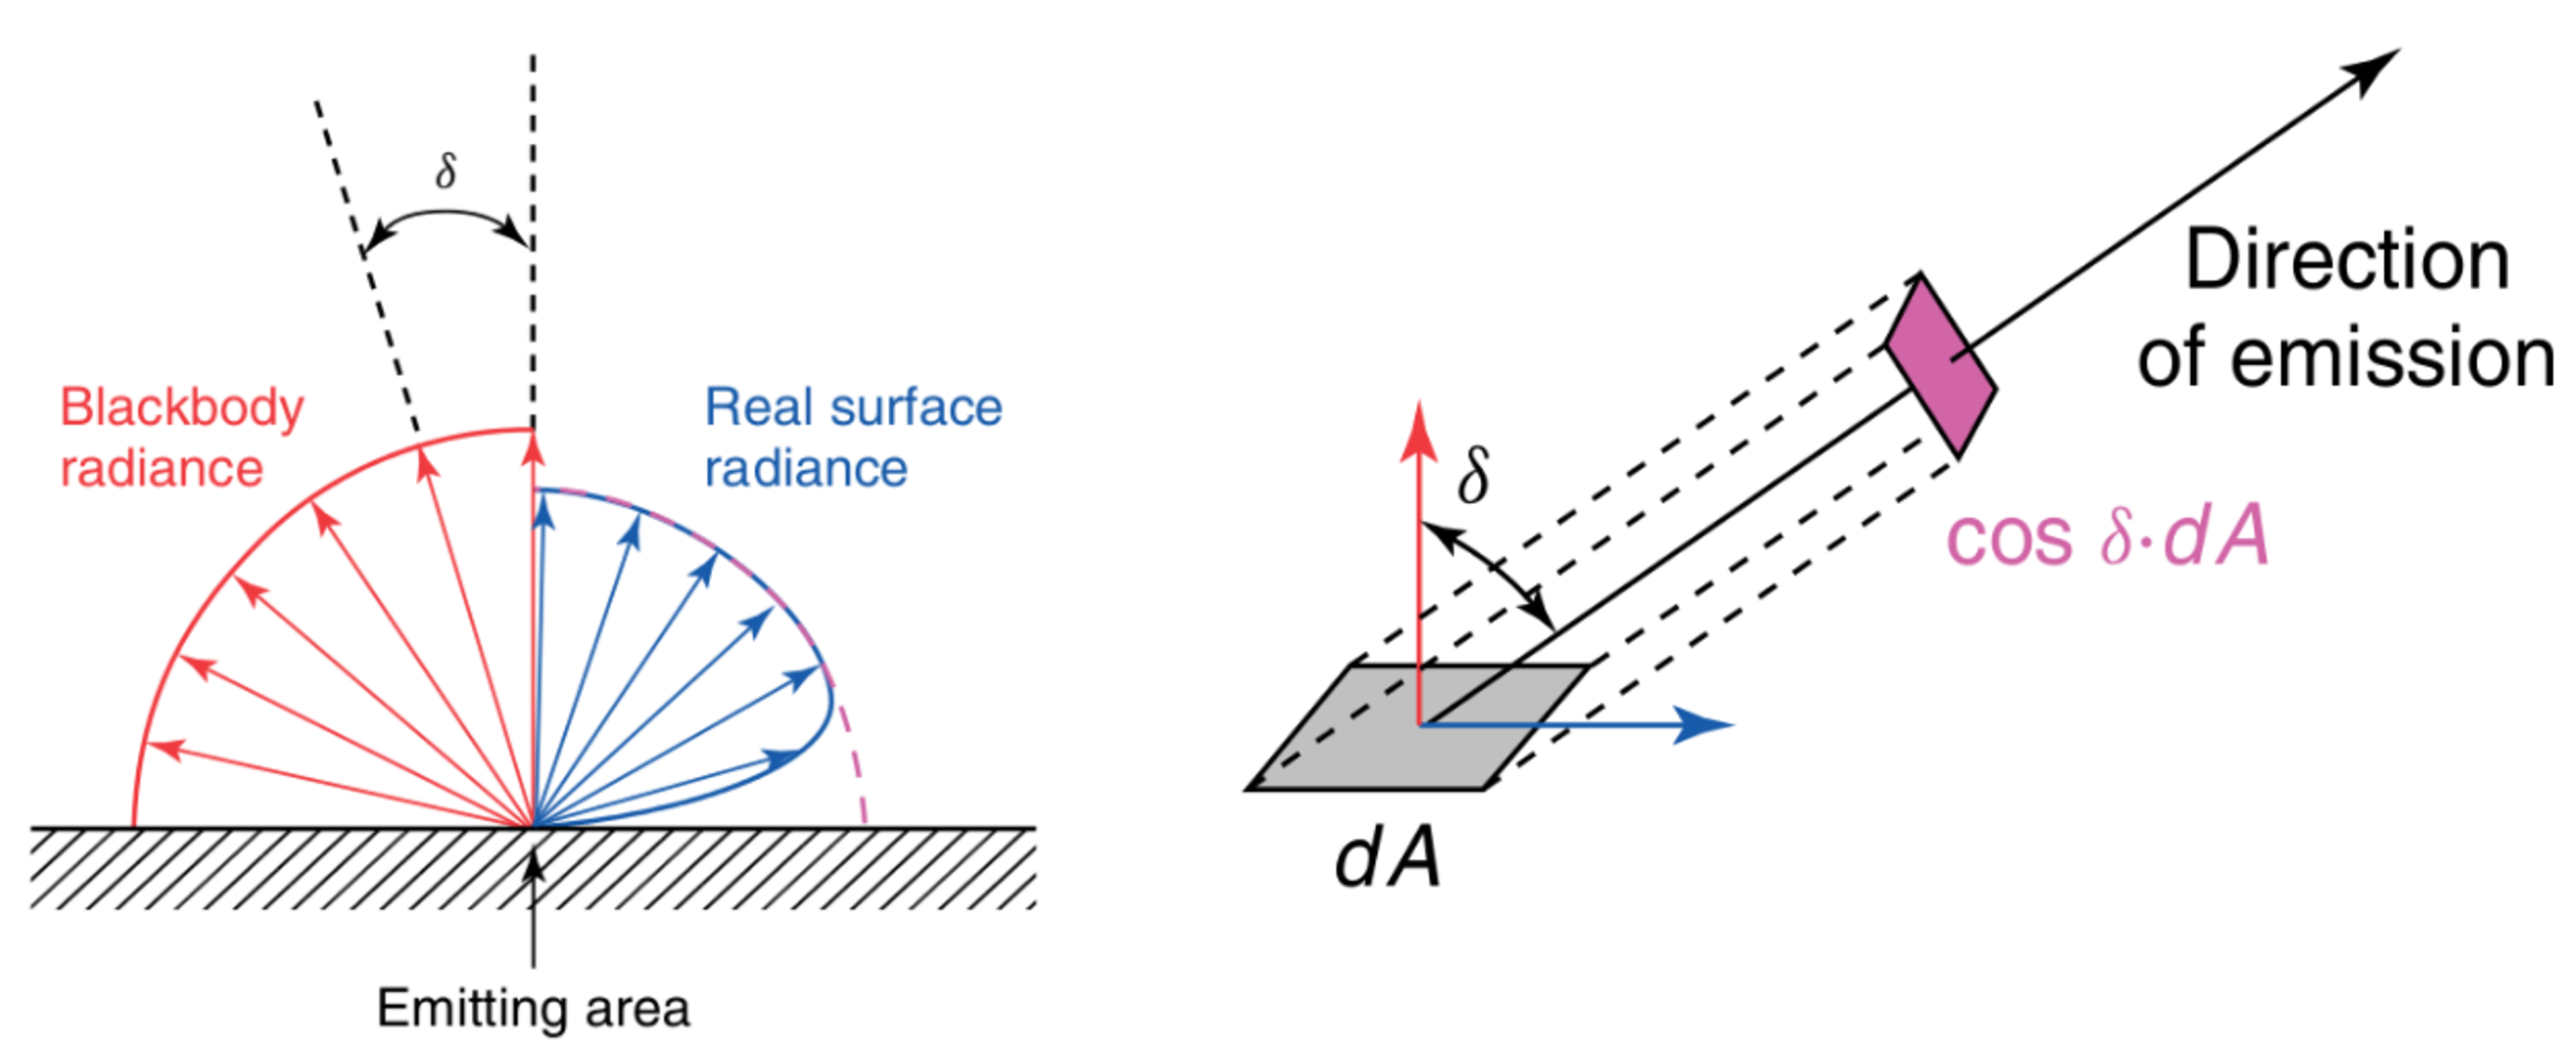
\includegraphics[scale=0.22]{Figures/Chapter03/AngularDistributionSchematics.pdf}
			\caption{Schematics of the angular dependence of the emissive power of a surface in relation to the blackbody}\label{fig3.2}
		\end{figure}
				
		Even though we can assume emissivity as a constant that only depends on the specific material of the surface under investigation, in general, it also depends on the viewing angle of the camera with respect to the normal of the surface. Blackbodies behave like perfect isotropically diffuse emitters, that is, for any surface emitting radiation, the radiance of the emitted radiation is independent of the direction into which it is emitted [8]. However, real surfaces, in addition to the lower emission rate (given by lower emissivity) also show angular dependence in the emissive power (Figure \ref{fig3.2} left).
		
		Usually, depending on the surface, the intensity of the emitted radiation might follow a cosine law with good approximation (Lambertian emitters). However, in general, this is not the case, and in most cases a study must be carried out to estimate the angular dependence of the emissivity [9, 10]. In order to determine whether this is a determining factor in our analysis, an angular study was performed using an aluminum rod filled with hot water placed in the same position as the Petal and, using a strip of high emissivity black tape along the rod's frontal face we were able to measure the variations in temperature due to the viewing angle (Figure \ref{fig3.3}).
				
		\begin{figure}[ht!]
			\centering
			\captionsetup{justification=centering,margin=2cm}
			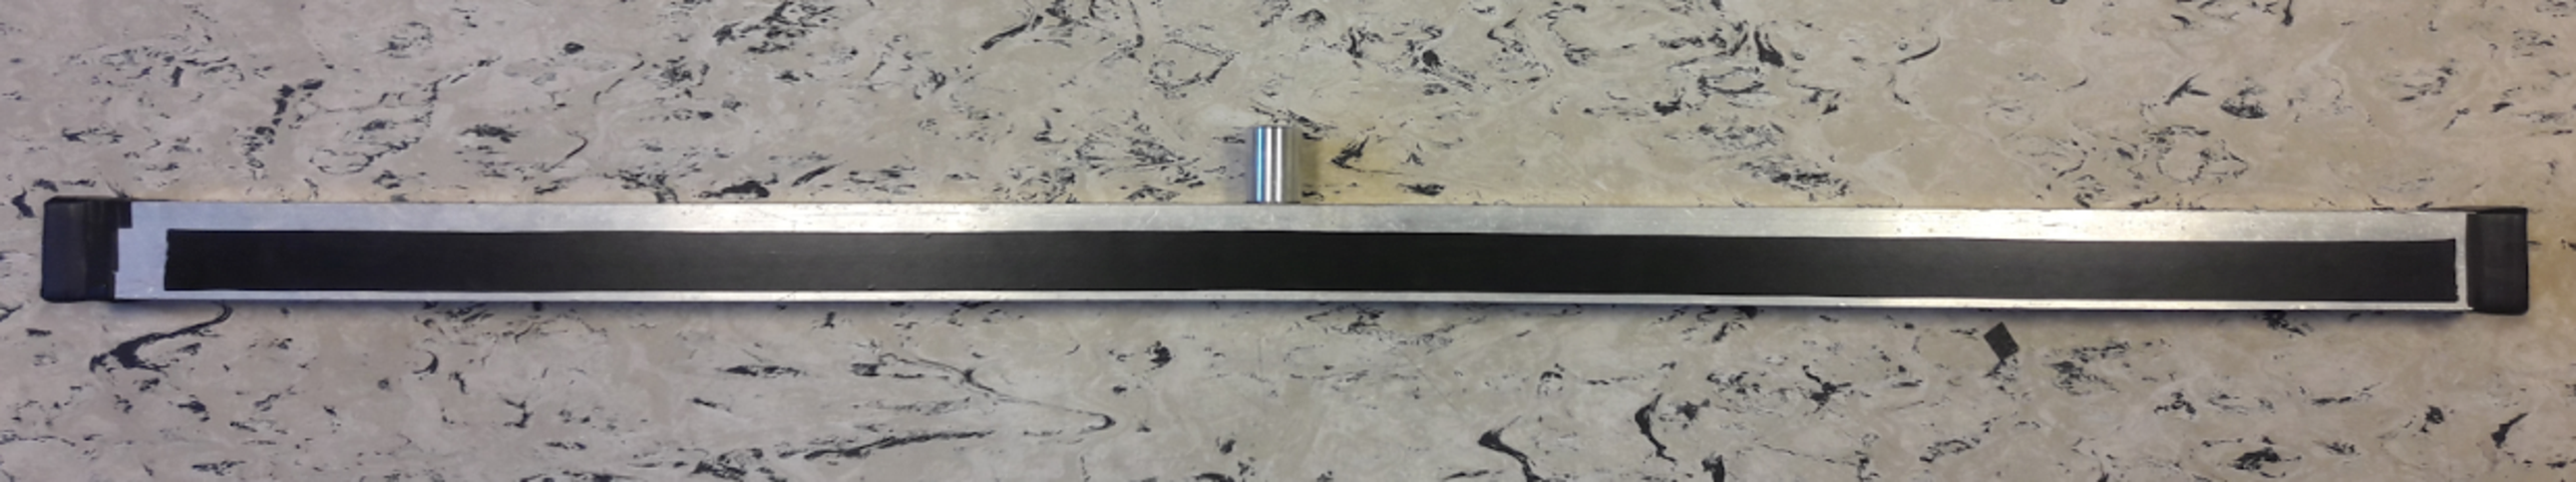
\includegraphics[scale=0.3]{Figures/Chapter03/AluminumRod.pdf}
			\caption{Aluminum rod used to study the angular dependence of emissivity.}\label{fig3.3}
		\end{figure}
		
		Of course, a combination of all the aforementioned factors leads to the small (but appreciable) differences between several materials in the image despite the fact that they are all at the same temperature. Figure \ref{fig3.4} shows an example of this effects in the emissive power perceived by the IR camera. This image is the ratio of the thermogram collected with the IR camera corresponding to the polished side of the Petal at room temperature (24.4 $^\circ C$ = 297.6 K) with no electronics powered on and no coolant flushed in and a thermogram where all the pixels have the same temperature of 297.6 K. This image clearly shows differences in temperatures among the different materials making visible the shape of the Petal itself. However, under ideal conditions, we shouldn't be able to distinguish any color variation since everything is supposed to be at the same temperature, that is, we should only see pixels with values of 1.
		
		\begin{figure}[ht!]
			\centering
			\captionsetup{justification=centering,margin=2cm}
			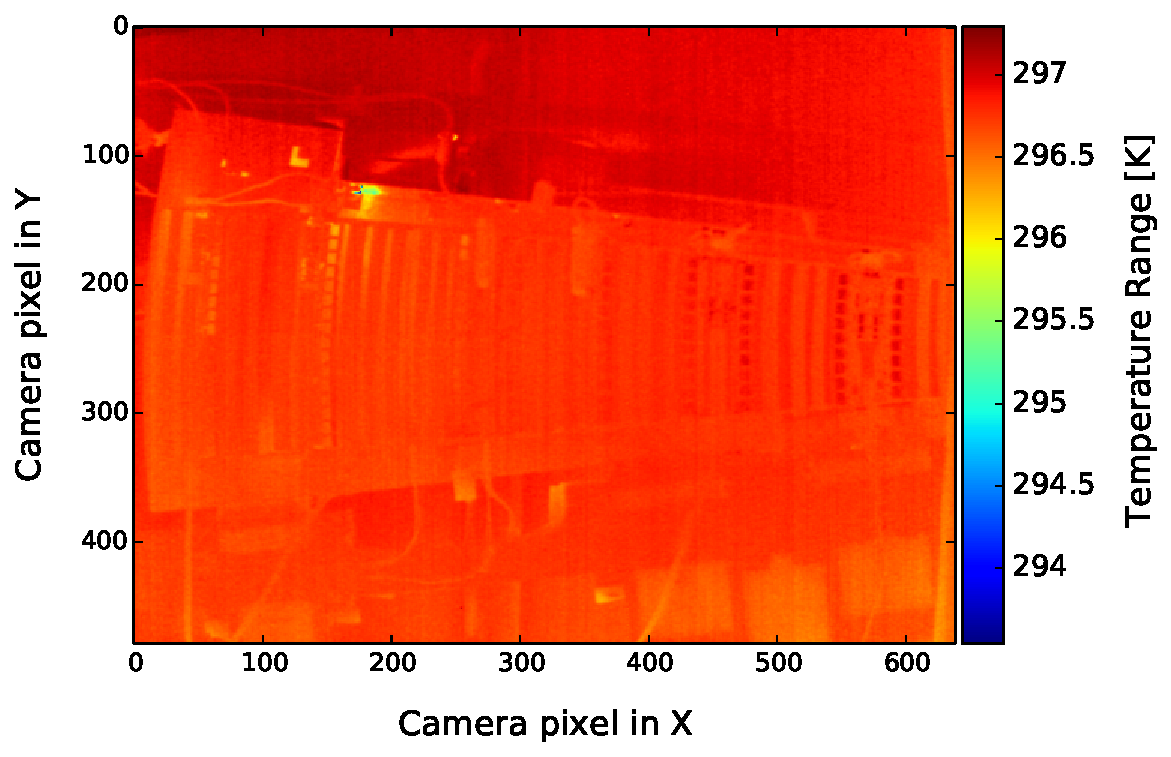
\includegraphics[scale=0.5]{Figures/Chapter03/thermo_Temp_201708091701_avg.pdf}
			\caption{Ratio thermogram of the Petal at room temperature. If the IR camera were 100\% accurate we should see all pixels with a ratio value of 1.}\label{fig3.4}
		\end{figure}
	
		\subsection{Apparent reflected temperature estimation.}\label{section3.1.1}
	
		\subsection{Emissivity estimation. Viewing angle influence.}\label{section3.1.2}
		
		\subsection{IR camera spectral response.}\label{section3.1.3}
		
		
	